\documentclass[tikz,border=12pt]{standalone}
\usepackage[T1]{fontenc}
\usepackage{mathpazo}
\usepackage{amsmath,amssymb}
\usetikzlibrary{arrows.meta, positioning, calc, fit, patterns, decorations.pathreplacing}

\definecolor{stblue}{HTML}{7B97AD}
\definecolor{rwgold}{HTML}{B8995E}
\definecolor{sage}{HTML}{7A9A7E}
\definecolor{dkbrown}{HTML}{3D3530}
\definecolor{wmgray}{HTML}{7B7067}
\definecolor{cream}{HTML}{F9F6F0}
\definecolor{border}{HTML}{D4C9B8}
\definecolor{terracotta}{HTML}{C47A6A}
\definecolor{lavender}{HTML}{907EA0}

\begin{document}
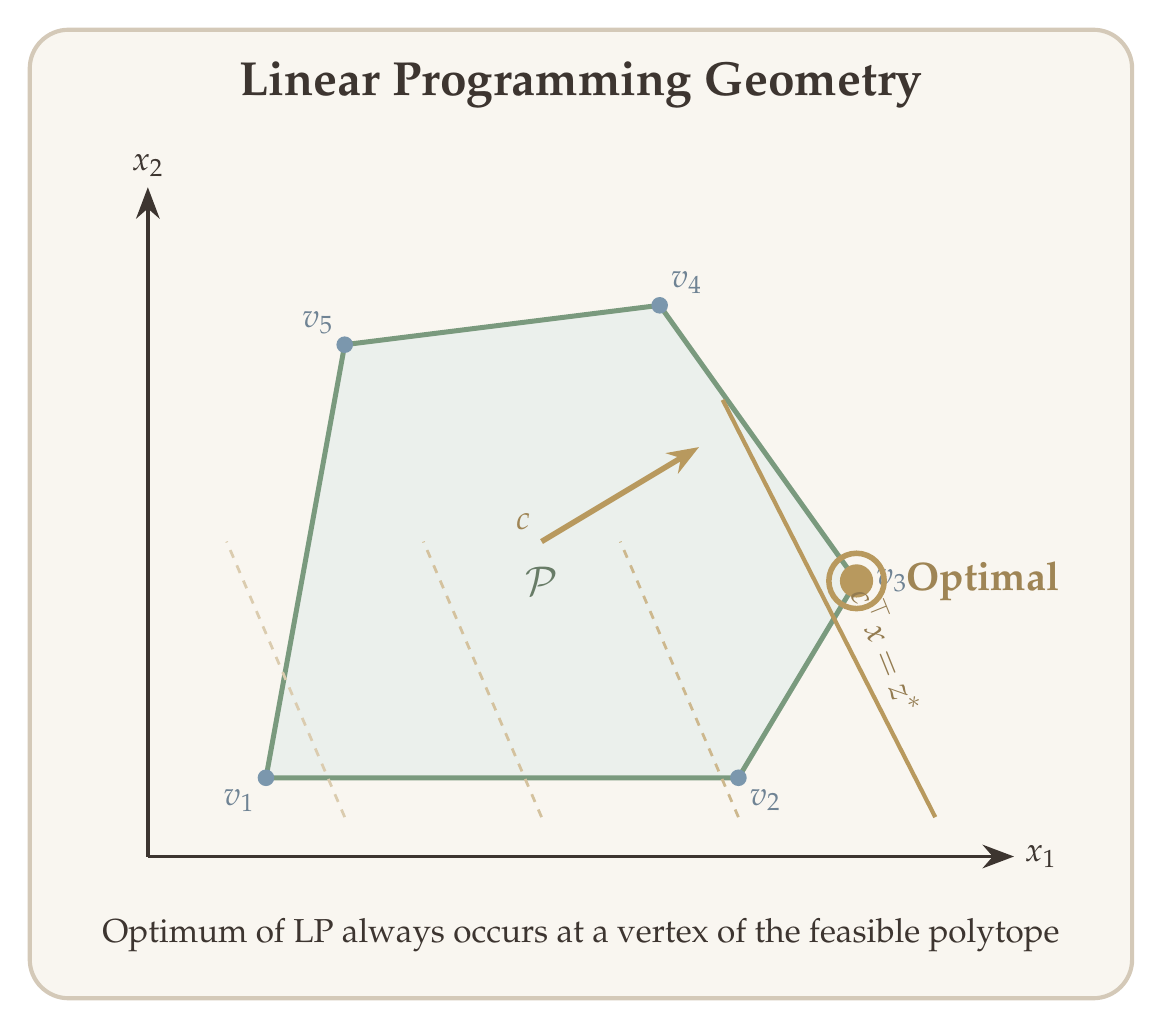
\begin{tikzpicture}[>={Stealth[length=4mm, width=3mm]}, line width=1.5pt]

% Background
\fill[cream, rounded corners=14pt] (-1,-1.8) rectangle (13,10.5);
\draw[border, line width=1.5pt, rounded corners=14pt] (-1,-1.8) rectangle (13,10.5);

% Title
\node[font=\LARGE\bfseries, text=dkbrown] at (6,9.8) {Linear Programming Geometry};

% Axes
\draw[->, dkbrown, line width=1.2pt] (0.5,0) -- (11.5,0) node[right, font=\large, text=dkbrown] {$x_1$};
\draw[->, dkbrown, line width=1.2pt] (0.5,0) -- (0.5,8.5) node[above, font=\large, text=dkbrown] {$x_2$};

% Feasible region (polygon)
\coordinate (v1) at (2,1);
\coordinate (v2) at (8,1);
\coordinate (v3) at (9.5,3.5);
\coordinate (v4) at (7,7);
\coordinate (v5) at (3,6.5);

\fill[sage!15] (v1) -- (v2) -- (v3) -- (v4) -- (v5) -- cycle;
\draw[sage, line width=1.8pt] (v1) -- (v2) -- (v3) -- (v4) -- (v5) -- cycle;

% Vertex labels
\fill[stblue] (v1) circle (3pt);
\node[font=\large, text=stblue!80!dkbrown, below left] at (v1) {$v_1$};
\fill[stblue] (v2) circle (3pt);
\node[font=\large, text=stblue!80!dkbrown, below right] at (v2) {$v_2$};
\fill[stblue] (v3) circle (3pt);
\node[font=\large, text=stblue!80!dkbrown, right=3pt] at (v3) {$v_3$};
\fill[stblue] (v4) circle (3pt);
\node[font=\large, text=stblue!80!dkbrown, above right] at (v4) {$v_4$};
\fill[stblue] (v5) circle (3pt);
\node[font=\large, text=stblue!80!dkbrown, above left] at (v5) {$v_5$};

% Optimal vertex (highlighted)
\fill[rwgold] (v3) circle (6pt);
\draw[rwgold, line width=2pt] (v3) circle (10pt);
\node[font=\Large\bfseries, text=rwgold!80!dkbrown, right=14pt] at (v3) {Optimal};

% Objective function direction arrow
\draw[->, rwgold, line width=2pt] (5.5,4) -- (7.5,5.2);
\node[font=\large, text=rwgold!80!dkbrown, above left] at (5.5,4) {$c$};

% Isoprofit lines
\draw[rwgold!50, line width=1pt, dashed] (3,0.5) -- (1.5,4);
\draw[rwgold!60, line width=1pt, dashed] (5.5,0.5) -- (4,4);
\draw[rwgold!70, line width=1pt, dashed] (8,0.5) -- (6.5,4);
% Isoprofit line touching optimal
\draw[rwgold, line width=1.5pt] (10.5,0.5) -- (7.8,5.8);
\node[font=\large, text=rwgold!70!dkbrown, rotate=-68, above] at (9.6,2.5) {$c^\top x = z^*$};

% Feasible region label
\node[font=\Large, text=sage!70!dkbrown] at (5.5,3.5) {$\mathcal{P}$};

% Legend
\node[font=\large, text=dkbrown] at (6,-1.0)
  {Optimum of LP always occurs at a vertex of the feasible polytope};

\end{tikzpicture}
\end{document}
